                        
\documentclass[a4paper]{article}
\usepackage[spanish]{babel}
\usepackage[utf8]{inputenc}
\usepackage{charter}   % tipografia
\usepackage{graphicx}
\usepackage{courier}
\usepackage{paralist} %itemize inline

\usepackage{amsmath, amsthm, amssymb}
%\lstset{language=C}

\usepackage{tipa}

\usepackage{color} % para snipets de codigo coloreados
\usepackage{fancybox}  % para el sbox de los snipets de codigo

\definecolor{litegrey}{gray}{0.94}

% \newenvironment{sidebar}{%
% 	\begin{Sbox}\begin{minipage}{.85\textwidth}}%
% 	{\end{minipage}\end{Sbox}%
% 		\begin{center}\setlength{\fboxsep}{6pt}%
% 		\shadowbox{\TheSbox}\end{center}}
% \newenvironment{warning}{%
% 	\begin{Sbox}\begin{minipage}{.85\textwidth}\sffamily\lite\small\RaggedRight}%
% 	{\end{minipage}\end{Sbox}%
% 		\begin{center}\setlength{\fboxsep}{6pt}%
% 		\colorbox{litegrey}{\TheSbox}\end{center}}

\newenvironment{codesnippet}{%
	\begin{Sbox}\begin{minipage}{\textwidth}\sffamily\small}%
	{\end{minipage}\end{Sbox}%
		\begin{center}%
		\vspace{-0.4cm}\colorbox{litegrey}{\TheSbox}\end{center}\vspace{0.3cm}}
\input{page.layout}
\usepackage{underscore}
\usepackage{caratula}
\usepackage{url}
\usepackage{enumitem}
\newcommand{\tab}{\hspace*{7mm}}

\usepackage{listings}
\lstset{
    language=C++,
    basewidth=0.55em,
    backgroundcolor=\color[rgb]{0.95,0.95,0.92},
    morekeywords={time_point,system_clock,duration}
}

\begin{document}

\thispagestyle{empty}
\materia{Bases de datos}
\submateria{Primer Cuatrimestre de 2017}
\titulo{Trabajo Práctico 1}
\grupo{Grupo 4}
\integrante{De Carli, Nicolás}{715/13}{nikodecarli@gmail.com}
\integrante{Gásperi, Fernando}{56/09}{fgasperijabalera@gmail.com}
\integrante{Gambaccini, Ezequiel}{164/13}{ezequiel.gambaccini@gmail.com}
\integrante{Minces, Javier}{231/13}{javier.minces@gmail.com}
\maketitle
\newpage

\tableofcontents

\newpage

\section{Introducción}

En este trabajo práctico presentaremos el diseño de una base de datos para la inscripción en un mundial de taekwondo. Debemos guardar los datos correspondientes a los competidores, coaches y árbitros, y los resultados obtenidos en cada categoría de cada modalidad.

En primer lugar mostraremos el diagrama entidad-relación, junto con las restricciones y suposiciones expresadas en lenguaje natural. Luego presentaremos el modelo relacional derivado, con el que se hará la base de datos real en MySQL.

\section{Diagrama Entidad Relación}

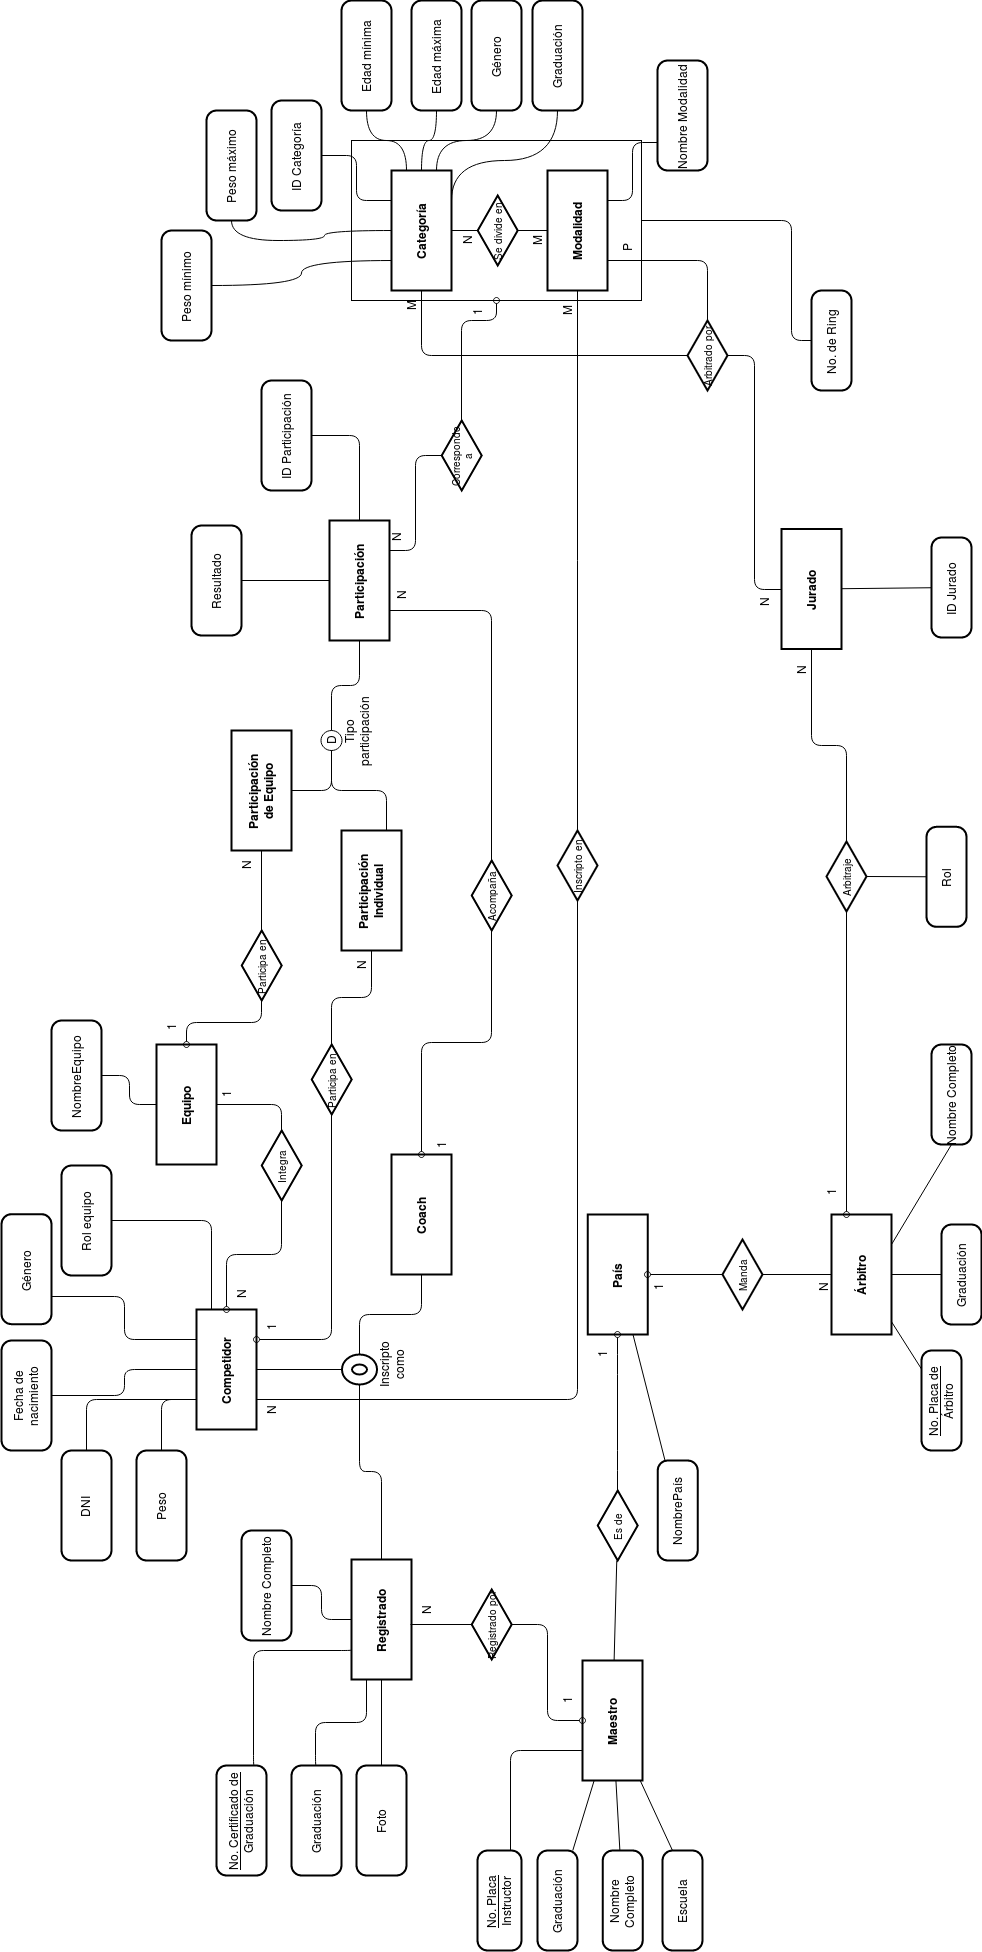
\includegraphics[height = \textheight]{mundialtaekwondo.png}

\section{Modelo Relacional}

Maestro(PlacaInstructor, Escuela, Nombre Completo, Graduacion, NombrePais)

País(NombrePais)

Árbitro(PlacaArbitro, Graduacion, Nombre Completo, NombrePais)

Arbitraje(IDJurado, PlacaArbitro, Rol)

Jurado(IDJurado)

ArbitradoPor(NombreModalidad, IDCategoria, IDJurado)

Modalidad(NombreModalidad)

Categoría(IDCategoria, Graduacion, EdadMinima, EdadMaxima, Sexo, PesoMinimo, PesoMaximo)

SeDivideEn(IDCategoria, NombreModalidad, Ring)

Registrado(NumeroCertificadoGraduacion, Foto,
Graduacion, NombreCompleto, PlacaInstructor)

Competidor(NumeroCertificadoGraduacion, Peso, DNI, FechaNacimiento, Genero, RolEquipo, NombreEquipo)

Coach(NumeroCertificadoGraduacion)

InscriptoEn(NumeroCertificadoGraduacion, NombreModalidad)

Equipo(NombreEquipo)

Participación(IDParticipacion, Resultado, IDCategoria, NombreModalidad, NumeroCertificadoGraduacionCoach, Tipo)

ParticipaciónIndividual(IDParticipacion, NumeroCertificadoGraduacionCompetidor)
ParticipaciónDeEquipo(IDParticipacion, NombreEquipo)

\subsection{Restricciones}

\begin{itemize}

\item La cantidad de coaches de una escuela debe ser 1/5 de la cantidad de alumnos

\item La graduación va de 1er dan a 6to dan

\item Para toda participación:

\item Si la categoría tiene peso máximo y mínimo el peso del competidor debe estar en el rango

\item Si la categoría tiene edad máxima y mínima la edad del competidor debe estar en el rango

\item Si la categoría tiene género el competidor debe ser de ese género

\item Si la categoría tiene graduación el competidor debe ser de esa graduación

\item Todos los integrantes de un equipo deben estar inscriptos en la modalidad combate por equipos

\item Los equipos deben tener 5 integrantes cuyo rol sea “titular” y 3 cuyo rol sea “suplente”

\item Todos los integrantes de un equipo deben ser de la misma escuela

\item Todos los integrantes de un equipo deben ser del mismo género, que debe corresponder con el género de la categoría de su participación por equipo.

\item Las participaciones de equipo deben ser en la modalidad “combate por equipos”.

\item Las participaciones individuales no pueden ser en la modalidad “combate por equipos”.

\item Cada competidor no puede tener más de una participación por modalidad

\item En cada jurado hay:

\item un árbitro con rol “presidente de mesa”

\item un “árbitro central”

\item dos o más “jueces”

\item tres o más “suplentes”.

\item La graduación de cada árbitro debe ser superior a la graduación de las categorías en las que es jurado. 

\item El coach de una participación debe ser de la misma escuela que el competidor

\end{itemize}

\section{Código}

\subsection{Creación de tablas}

\lstinputlisting[language=sql, breaklines = true]{createtables.sql}

\subsection{Restricciones - triggers}

\lstinputlisting[language=sql, breaklines = true]{additionalconstraints.tex}

\subsection{Restricciones - stored procedure}

\lstinputlisting[language=sql, breaklines = true]{storeprocedureinsert.sql}

\subsection{Queries}

\lstinputlisting[language=sql, breaklines = true]{queries.sql}

\section{Conclusión}

\newpage

\end{document}
